% Diagrama de atividades do cancelamento e do reagendamento. Gera AtividadeCancelaa.png.
\documentclass[border=8pt]{standalone}
\usepackage[utf8]{inputenc}
\usepackage[T1]{fontenc}
\usepackage{tikz}
\usetikzlibrary{shapes.geometric,positioning,arrows.meta,calc}
\tikzset{
  acao/.style={rectangle, rounded corners=5pt, draw, text width=4.6cm, align=center,
    minimum height=0.85cm, inner sep=4pt},
  lado/.style={acao, text width=2.9cm},
  decisao/.style={diamond, aspect=2.6, draw, text width=3.3cm, align=center, inner sep=-1pt},
  inicio/.style={circle, fill=black, minimum size=0.5cm, inner sep=0pt},
  fim/.style={circle, draw, double, double distance=1.2pt, fill=black, minimum size=0.45cm, inner sep=0pt},
  seta/.style={-{Latex[length=2.2mm]}},
  rot/.style={font=\small},
}
\begin{document}
\hyphenpenalty=10000\exhyphenpenalty=10000
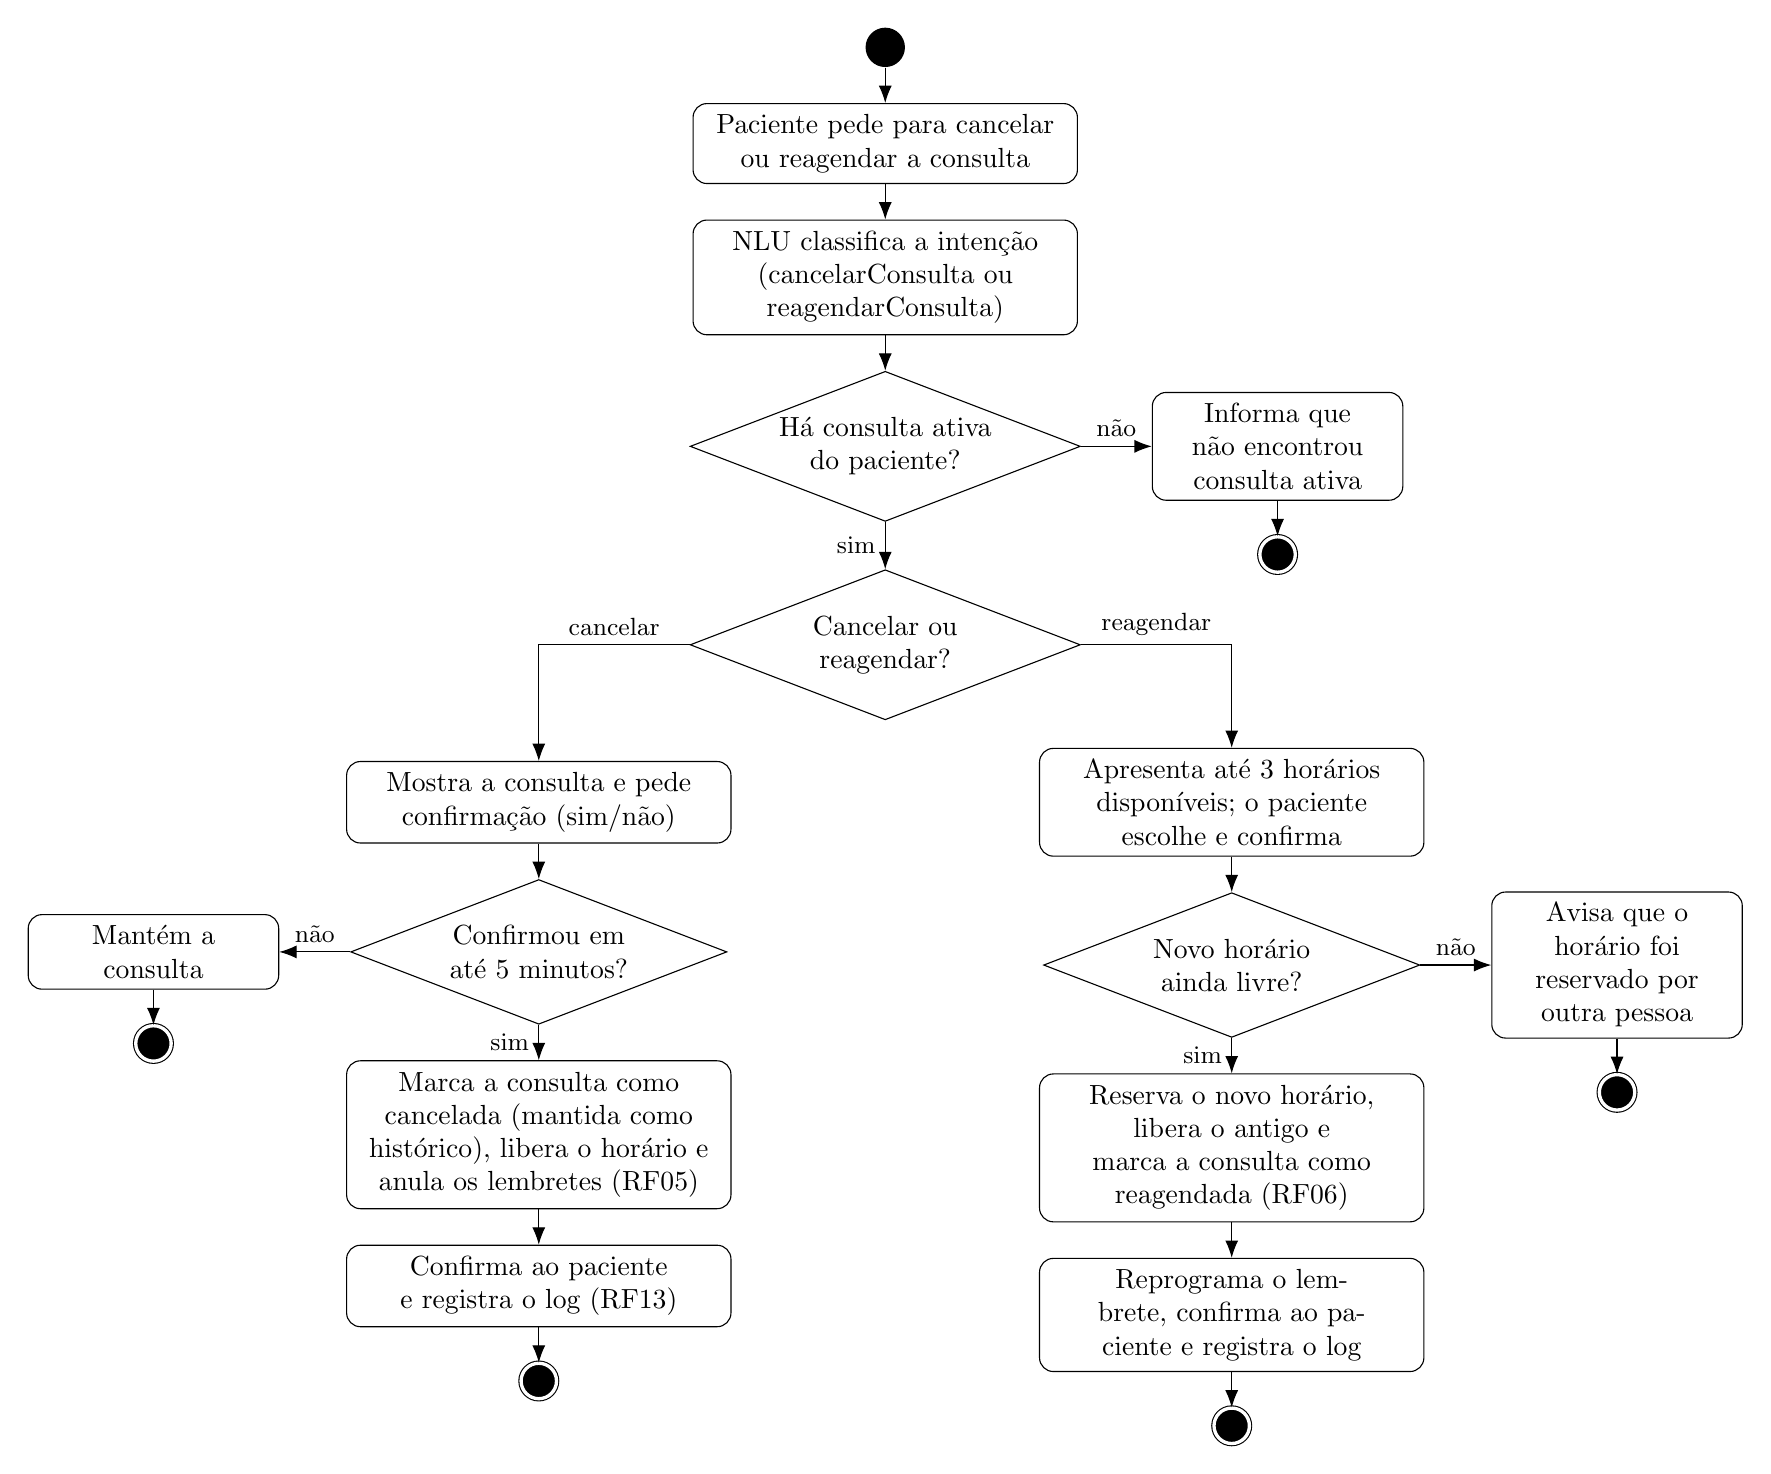
\begin{tikzpicture}[node distance=0.45cm and 0.9cm]
% tronco comum
\node[inicio] (ini) at (0,0) {};
\node[acao, below=of ini] (pede) {Paciente pede para cancelar ou reagendar a consulta};
\node[acao, below=of pede] (nlu) {NLU classifica a intenção (cancelarConsulta ou reagendarConsulta)};
\node[decisao, below=of nlu] (ativa) {Há consulta ativa do paciente?};
\node[lado, right=of ativa] (naoachou) {Informa que não encontrou consulta ativa};
\node[fim, below=of naoachou] (f0) {};
\node[decisao, below=0.6cm of ativa] (qual) {Cancelar ou \\ reagendar?};

% cancelamento (coluna da esquerda)
\node[acao] (mostra) at ($(qual)+(-4.4,-2.0)$) {Mostra a consulta e pede confirmação (sim/não)};
\node[decisao, below=of mostra] (confirmou) {Confirmou em até 5 minutos?};
\node[lado, left=of confirmou] (mantem) {Mantém a consulta};
\node[fim, below=of mantem] (f1) {};
\node[acao, below=of confirmou] (cancela) {Marca a consulta como cancelada (mantida como histórico), libera o horário e anula os lembretes (RF05)};
\node[acao, below=of cancela] (confc) {Confirma ao paciente e registra o log (RF13)};
\node[fim, below=of confc] (f2) {};

% reagendamento (coluna da direita)
\node[acao] (opcoes) at ($(qual)+(4.4,-2.0)$) {Apresenta até 3 horários disponíveis; o paciente escolhe e confirma};
\node[decisao, below=of opcoes] (livre) {Novo horário ainda livre?};
\node[lado, right=of livre] (tomado) {Avisa que o horário foi reservado por outra pessoa};
\node[fim, below=of tomado] (f3) {};
\node[acao, below=of livre] (reag) {Reserva o novo horário, libera o antigo e marca a consulta como reagendada (RF06)};
\node[acao, below=of reag] (confr) {Reprograma o lembrete, confirma ao paciente e registra o log};
\node[fim, below=of confr] (f4) {};

\draw[seta] (ini) -- (pede);
\draw[seta] (pede) -- (nlu);
\draw[seta] (nlu) -- (ativa);
\draw[seta] (ativa) -- node[rot,above]{não} (naoachou);
\draw[seta] (naoachou) -- (f0);
\draw[seta] (ativa) -- node[rot,left]{sim} (qual);
\draw[seta] (qual.west) -| node[rot,above,pos=0.25]{cancelar} (mostra.north);
\draw[seta] (qual.east) -| node[rot,above,pos=0.25]{reagendar} (opcoes.north);
\draw[seta] (mostra) -- (confirmou);
\draw[seta] (confirmou) -- node[rot,above]{não} (mantem);
\draw[seta] (mantem) -- (f1);
\draw[seta] (confirmou) -- node[rot,left]{sim} (cancela);
\draw[seta] (cancela) -- (confc);
\draw[seta] (confc) -- (f2);
\draw[seta] (opcoes) -- (livre);
\draw[seta] (livre) -- node[rot,above]{não} (tomado);
\draw[seta] (tomado) -- (f3);
\draw[seta] (livre) -- node[rot,left]{sim} (reag);
\draw[seta] (reag) -- (confr);
\draw[seta] (confr) -- (f4);
\end{tikzpicture}
\end{document}
